\documentclass[twoside]{book}

% Packages required by doxygen
\usepackage{fixltx2e}
\usepackage{calc}
\usepackage{doxygen}
\usepackage[export]{adjustbox} % also loads graphicx
\usepackage{graphicx}
\usepackage[utf8]{inputenc}
\usepackage{makeidx}
\usepackage{multicol}
\usepackage{multirow}
\PassOptionsToPackage{warn}{textcomp}
\usepackage{textcomp}
\usepackage[nointegrals]{wasysym}
\usepackage[table]{xcolor}

% Font selection
\usepackage[T1]{fontenc}
\usepackage[scaled=.90]{helvet}
\usepackage{courier}
\usepackage{amssymb}
\usepackage{sectsty}
\renewcommand{\familydefault}{\sfdefault}
\allsectionsfont{%
  \fontseries{bc}\selectfont%
  \color{darkgray}%
}
\renewcommand{\DoxyLabelFont}{%
  \fontseries{bc}\selectfont%
  \color{darkgray}%
}
\newcommand{\+}{\discretionary{\mbox{\scriptsize$\hookleftarrow$}}{}{}}

% Page & text layout
\usepackage{geometry}
\geometry{%
  a4paper,%
  top=2.5cm,%
  bottom=2.5cm,%
  left=2.5cm,%
  right=2.5cm%
}
\tolerance=750
\hfuzz=15pt
\hbadness=750
\setlength{\emergencystretch}{15pt}
\setlength{\parindent}{0cm}
\setlength{\parskip}{3ex plus 2ex minus 2ex}
\makeatletter
\renewcommand{\paragraph}{%
  \@startsection{paragraph}{4}{0ex}{-1.0ex}{1.0ex}{%
    \normalfont\normalsize\bfseries\SS@parafont%
  }%
}
\renewcommand{\subparagraph}{%
  \@startsection{subparagraph}{5}{0ex}{-1.0ex}{1.0ex}{%
    \normalfont\normalsize\bfseries\SS@subparafont%
  }%
}
\makeatother

% Headers & footers
\usepackage{fancyhdr}
\pagestyle{fancyplain}
\fancyhead[LE]{\fancyplain{}{\bfseries\thepage}}
\fancyhead[CE]{\fancyplain{}{}}
\fancyhead[RE]{\fancyplain{}{\bfseries\leftmark}}
\fancyhead[LO]{\fancyplain{}{\bfseries\rightmark}}
\fancyhead[CO]{\fancyplain{}{}}
\fancyhead[RO]{\fancyplain{}{\bfseries\thepage}}
\fancyfoot[LE]{\fancyplain{}{}}
\fancyfoot[CE]{\fancyplain{}{}}
\fancyfoot[RE]{\fancyplain{}{\bfseries\scriptsize Generated by Doxygen }}
\fancyfoot[LO]{\fancyplain{}{\bfseries\scriptsize Generated by Doxygen }}
\fancyfoot[CO]{\fancyplain{}{}}
\fancyfoot[RO]{\fancyplain{}{}}
\renewcommand{\footrulewidth}{0.4pt}
\renewcommand{\chaptermark}[1]{%
  \markboth{#1}{}%
}
\renewcommand{\sectionmark}[1]{%
  \markright{\thesection\ #1}%
}

% Indices & bibliography
\usepackage{natbib}
\usepackage[titles]{tocloft}
\setcounter{tocdepth}{3}
\setcounter{secnumdepth}{5}
\makeindex

% Hyperlinks (required, but should be loaded last)
\usepackage{ifpdf}
\ifpdf
  \usepackage[pdftex,pagebackref=true]{hyperref}
\else
  \usepackage[ps2pdf,pagebackref=true]{hyperref}
\fi
\hypersetup{%
  colorlinks=true,%
  linkcolor=blue,%
  citecolor=blue,%
  unicode%
}

% Custom commands
\newcommand{\clearemptydoublepage}{%
  \newpage{\pagestyle{empty}\cleardoublepage}%
}

\usepackage{caption}
\captionsetup{labelsep=space,justification=centering,font={bf},singlelinecheck=off,skip=4pt,position=top}

%===== C O N T E N T S =====

\begin{document}

% Titlepage & ToC
\hypersetup{pageanchor=false,
             bookmarksnumbered=true,
             pdfencoding=unicode
            }
\pagenumbering{roman}
\begin{titlepage}
\vspace*{7cm}
\begin{center}%
{\Large My Project }\\
\vspace*{1cm}
{\large Generated by Doxygen 1.8.11}\\
\end{center}
\end{titlepage}
\clearemptydoublepage
\tableofcontents
\clearemptydoublepage
\pagenumbering{arabic}
\hypersetup{pageanchor=true}

%--- Begin generated contents ---
\chapter{Class Index}
\section{Class List}
Here are the classes, structs, unions and interfaces with brief descriptions\+:\begin{DoxyCompactList}
\item\contentsline{section}{\hyperlink{class_boid}{Boid} }{\pageref{class_boid}}{}
\item\contentsline{section}{\hyperlink{class_flock}{Flock} }{\pageref{class_flock}}{}
\item\contentsline{section}{\hyperlink{class_game}{Game} }{\pageref{class_game}}{}
\item\contentsline{section}{\hyperlink{class_pvector}{Pvector} }{\pageref{class_pvector}}{}
\end{DoxyCompactList}

\chapter{Class Documentation}
\hypertarget{class_boid}{}\section{Boid Class Reference}
\label{class_boid}\index{Boid@{Boid}}


{\ttfamily \#include $<$Boid.\+h$>$}



Collaboration diagram for Boid\+:
\nopagebreak
\begin{figure}[H]
\begin{center}
\leavevmode
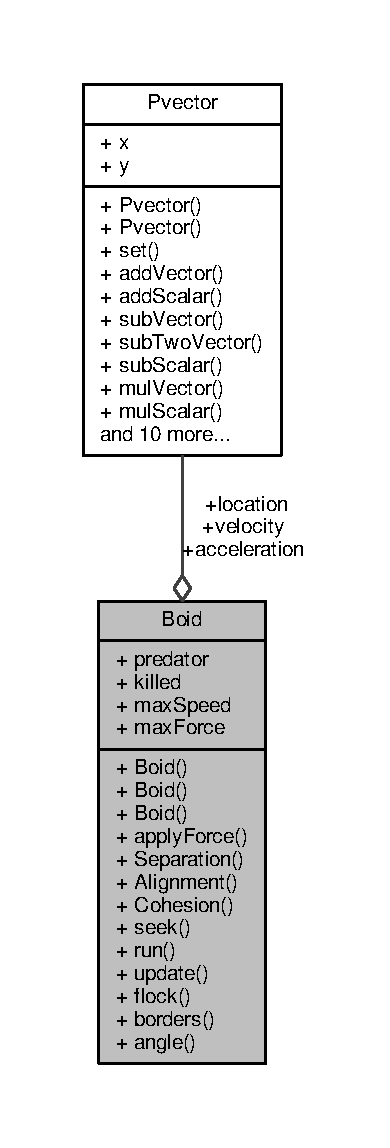
\includegraphics[height=550pt]{class_boid__coll__graph}
\end{center}
\end{figure}
\subsection*{Public Member Functions}
\begin{DoxyCompactItemize}
\item 
{\bfseries Boid} (float x, float y)\hypertarget{class_boid_a61c7081f12c16ba99dc4b3c094195bb2}{}\label{class_boid_a61c7081f12c16ba99dc4b3c094195bb2}

\item 
\hyperlink{class_boid_a22e47f71f5d635f788ff747cf69bdc55}{Boid} (float x, float y, int pred\+Check)\hypertarget{class_boid_a22e47f71f5d635f788ff747cf69bdc55}{}\label{class_boid_a22e47f71f5d635f788ff747cf69bdc55}

\begin{DoxyCompactList}\small\item\em \hyperlink{class_boid_acef10e100c27b76f6b867ae7468c09bb}{apply\+Force(\+Pvector force)}\+: Adds the given vector to acceleration \end{DoxyCompactList}\item 
void \hyperlink{class_boid_acef10e100c27b76f6b867ae7468c09bb}{apply\+Force} (\hyperlink{class_pvector}{Pvector} force)\hypertarget{class_boid_acef10e100c27b76f6b867ae7468c09bb}{}\label{class_boid_acef10e100c27b76f6b867ae7468c09bb}

\begin{DoxyCompactList}\small\item\em Three Laws that boids follow. \end{DoxyCompactList}\item 
\hyperlink{class_pvector}{Pvector} \hyperlink{class_boid_aa6910fba0e1edba1eac4c1ca234d1199}{Separation} (vector$<$ \hyperlink{class_boid}{Boid} $>$ Boids)
\item 
\hyperlink{class_pvector}{Pvector} \hyperlink{class_boid_ac1830d68d2af0eade8d26fc6084960aa}{Alignment} (vector$<$ \hyperlink{class_boid}{Boid} $>$ Boids)
\item 
\hyperlink{class_pvector}{Pvector} \hyperlink{class_boid_ae1f8d78202e983a11f1ee72e1de0473c}{Cohesion} (vector$<$ \hyperlink{class_boid}{Boid} $>$ Boids)
\begin{DoxyCompactList}\small\item\em Functions involving S\+F\+ML and visualisation linking. \end{DoxyCompactList}\item 
\hyperlink{class_pvector}{Pvector} {\bfseries seek} (\hyperlink{class_pvector}{Pvector} v)\hypertarget{class_boid_a3135a25087ac386d92e28b5718f6504f}{}\label{class_boid_a3135a25087ac386d92e28b5718f6504f}

\item 
void {\bfseries run} (vector$<$ \hyperlink{class_boid}{Boid} $>$ v)\hypertarget{class_boid_a292bf6dc850fe8d220fe3af7667e1090}{}\label{class_boid_a292bf6dc850fe8d220fe3af7667e1090}

\item 
void {\bfseries update} ()\hypertarget{class_boid_a7404d18dcb7dfc669e80c534819fa893}{}\label{class_boid_a7404d18dcb7dfc669e80c534819fa893}

\item 
void {\bfseries flock} (vector$<$ \hyperlink{class_boid}{Boid} $>$ v)\hypertarget{class_boid_ab8696c8548189dba88f59d917a2212fb}{}\label{class_boid_ab8696c8548189dba88f59d917a2212fb}

\item 
void {\bfseries borders} ()\hypertarget{class_boid_ab297036090d8dad9e70379ecfeb60137}{}\label{class_boid_ab297036090d8dad9e70379ecfeb60137}

\item 
float {\bfseries angle} (\hyperlink{class_pvector}{Pvector} v)\hypertarget{class_boid_afeb7353f3946b4bd1072a14aee888770}{}\label{class_boid_afeb7353f3946b4bd1072a14aee888770}

\end{DoxyCompactItemize}
\subsection*{Public Attributes}
\begin{DoxyCompactItemize}
\item 
int \hyperlink{class_boid_af6faa80aeac271c4521eca772336a8b9}{predator}
\begin{DoxyCompactList}\small\item\em $<$ bool predator\+: flag that specifies whether a given boid is a predator. \end{DoxyCompactList}\item 
int \hyperlink{class_boid_afb70f86fbd40056d76c7d3875d20e699}{killed}\hypertarget{class_boid_afb70f86fbd40056d76c7d3875d20e699}{}\label{class_boid_afb70f86fbd40056d76c7d3875d20e699}

\begin{DoxyCompactList}\small\item\em \hyperlink{class_pvector}{Pvector} location\+: Vector that specifies a boid\textquotesingle{}s location. \end{DoxyCompactList}\item 
\hyperlink{class_pvector}{Pvector} \hyperlink{class_boid_a92a7f1ed6423149cd8a28426695d127e}{location}\hypertarget{class_boid_a92a7f1ed6423149cd8a28426695d127e}{}\label{class_boid_a92a7f1ed6423149cd8a28426695d127e}

\begin{DoxyCompactList}\small\item\em \hyperlink{class_pvector}{Pvector} velocity\+: Vector that specifies a boid\textquotesingle{}s current velocity. \end{DoxyCompactList}\item 
\hyperlink{class_pvector}{Pvector} \hyperlink{class_boid_af79ca165b4d1a6ad1db2cbc534095bab}{velocity}\hypertarget{class_boid_af79ca165b4d1a6ad1db2cbc534095bab}{}\label{class_boid_af79ca165b4d1a6ad1db2cbc534095bab}

\begin{DoxyCompactList}\small\item\em \hyperlink{class_pvector}{Pvector} acceleration\+: Vector that specifies a boid\textquotesingle{}s current acceleration. \end{DoxyCompactList}\item 
\hyperlink{class_pvector}{Pvector} \hyperlink{class_boid_ac29a50172433e865b12e1023f00f90c0}{acceleration}\hypertarget{class_boid_ac29a50172433e865b12e1023f00f90c0}{}\label{class_boid_ac29a50172433e865b12e1023f00f90c0}

\begin{DoxyCompactList}\small\item\em float max\+Speed\+: Limits magnitude of velocity vector. \end{DoxyCompactList}\item 
float \hyperlink{class_boid_ac57e1058fb698a542990405ecfd1d88b}{max\+Speed}\hypertarget{class_boid_ac57e1058fb698a542990405ecfd1d88b}{}\label{class_boid_ac57e1058fb698a542990405ecfd1d88b}

\begin{DoxyCompactList}\small\item\em float max\+Force\+: Limits magnitude of acceleration vector. (F = m$\ast$a!) \end{DoxyCompactList}\item 
float \hyperlink{class_boid_a2a6d579118276efaeac7ba0e4b872afd}{max\+Force}\hypertarget{class_boid_a2a6d579118276efaeac7ba0e4b872afd}{}\label{class_boid_a2a6d579118276efaeac7ba0e4b872afd}

\begin{DoxyCompactList}\small\item\em boid constructor \end{DoxyCompactList}\end{DoxyCompactItemize}


\subsection{Detailed Description}
The \hyperlink{class_boid}{Boid} Class 

\subsection{Member Function Documentation}
\index{Boid@{Boid}!Alignment@{Alignment}}
\index{Alignment@{Alignment}!Boid@{Boid}}
\subsubsection[{\texorpdfstring{Alignment(vector$<$ Boid $>$ Boids)}{Alignment(vector< Boid > Boids)}}]{\setlength{\rightskip}{0pt plus 5cm}{\bf Pvector} Boid\+::\+Alignment (
\begin{DoxyParamCaption}
\item[{vector$<$ {\bf Boid} $>$}]{Boids}
\end{DoxyParamCaption}
)}\hypertarget{class_boid_ac1830d68d2af0eade8d26fc6084960aa}{}\label{class_boid_ac1830d68d2af0eade8d26fc6084960aa}
\hyperlink{class_pvector}{Pvector} \hyperlink{class_boid_ac1830d68d2af0eade8d26fc6084960aa}{Alignment(vector$<$\+Boid$>$ Boids)}\+: Computes a vector that causes the velocity of the current boid to match that of boids that are nearby. \index{Boid@{Boid}!Cohesion@{Cohesion}}
\index{Cohesion@{Cohesion}!Boid@{Boid}}
\subsubsection[{\texorpdfstring{Cohesion(vector$<$ Boid $>$ Boids)}{Cohesion(vector< Boid > Boids)}}]{\setlength{\rightskip}{0pt plus 5cm}{\bf Pvector} Boid\+::\+Cohesion (
\begin{DoxyParamCaption}
\item[{vector$<$ {\bf Boid} $>$}]{Boids}
\end{DoxyParamCaption}
)}\hypertarget{class_boid_ae1f8d78202e983a11f1ee72e1de0473c}{}\label{class_boid_ae1f8d78202e983a11f1ee72e1de0473c}


Functions involving S\+F\+ML and visualisation linking. 

\hyperlink{class_pvector}{Pvector} \hyperlink{class_boid_ae1f8d78202e983a11f1ee72e1de0473c}{Cohesion(vector$<$\+Boid$>$ Boids)}\+: Computes a vector that causes the current boid to seek the center of mass of nearby boids. \index{Boid@{Boid}!Separation@{Separation}}
\index{Separation@{Separation}!Boid@{Boid}}
\subsubsection[{\texorpdfstring{Separation(vector$<$ Boid $>$ Boids)}{Separation(vector< Boid > Boids)}}]{\setlength{\rightskip}{0pt plus 5cm}{\bf Pvector} Boid\+::\+Separation (
\begin{DoxyParamCaption}
\item[{vector$<$ {\bf Boid} $>$}]{Boids}
\end{DoxyParamCaption}
)}\hypertarget{class_boid_aa6910fba0e1edba1eac4c1ca234d1199}{}\label{class_boid_aa6910fba0e1edba1eac4c1ca234d1199}
\hyperlink{class_pvector}{Pvector} \hyperlink{class_boid_aa6910fba0e1edba1eac4c1ca234d1199}{Separation(vector$<$\+Boid$>$ Boids)}\+: If any other boids are within a given distance, Separation computes a a vector that distances the current boid from the boids that are too close. 

\subsection{Member Data Documentation}
\index{Boid@{Boid}!predator@{predator}}
\index{predator@{predator}!Boid@{Boid}}
\subsubsection[{\texorpdfstring{predator}{predator}}]{\setlength{\rightskip}{0pt plus 5cm}int Boid\+::predator}\hypertarget{class_boid_af6faa80aeac271c4521eca772336a8b9}{}\label{class_boid_af6faa80aeac271c4521eca772336a8b9}


$<$ bool predator\+: flag that specifies whether a given boid is a predator. 

bool killed\+: flag that specifies whether a given boid is alive. 

The documentation for this class was generated from the following file\+:\begin{DoxyCompactItemize}
\item 
Boid.\+h\end{DoxyCompactItemize}

\hypertarget{class_flock}{}\section{Flock Class Reference}
\label{class_flock}\index{Flock@{Flock}}


{\ttfamily \#include $<$Flock.\+h$>$}



Collaboration diagram for Flock\+:
\nopagebreak
\begin{figure}[H]
\begin{center}
\leavevmode
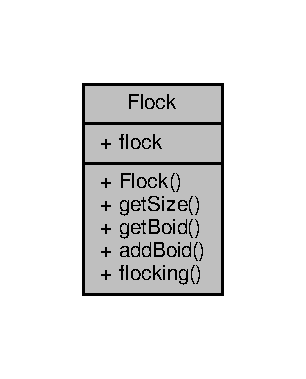
\includegraphics[width=147pt]{class_flock__coll__graph}
\end{center}
\end{figure}
\subsection*{Public Member Functions}
\begin{DoxyCompactItemize}
\item 
\hyperlink{class_flock_a2a0a514c368e21f718ad7358ed42f3b7}{Flock} ()\hypertarget{class_flock_a2a0a514c368e21f718ad7358ed42f3b7}{}\label{class_flock_a2a0a514c368e21f718ad7358ed42f3b7}

\begin{DoxyCompactList}\small\item\em Accessor functions. \end{DoxyCompactList}\item 
int {\bfseries get\+Size} ()\hypertarget{class_flock_ae5801b4eed7ae1e9719f50550424e8f1}{}\label{class_flock_ae5801b4eed7ae1e9719f50550424e8f1}

\item 
\hyperlink{class_boid}{Boid} \hyperlink{class_flock_a79925dd0c9568e57417d5d459711682d}{get\+Boid} (int i)\hypertarget{class_flock_a79925dd0c9568e57417d5d459711682d}{}\label{class_flock_a79925dd0c9568e57417d5d459711682d}

\begin{DoxyCompactList}\small\item\em Mutator Functions. \end{DoxyCompactList}\item 
void {\bfseries add\+Boid} (\hyperlink{class_boid}{Boid} b)\hypertarget{class_flock_ad671f2430e8b980c74d9654abe9acbc9}{}\label{class_flock_ad671f2430e8b980c74d9654abe9acbc9}

\item 
void {\bfseries flocking} ()\hypertarget{class_flock_a90c029c6cacb19193dd0b94ad74900e7}{}\label{class_flock_a90c029c6cacb19193dd0b94ad74900e7}

\end{DoxyCompactItemize}
\subsection*{Public Attributes}
\begin{DoxyCompactItemize}
\item 
vector$<$ \hyperlink{class_boid}{Boid} $>$ \hyperlink{class_flock_a5f82ca864e51913c633c2a75fe8ba854}{flock}\hypertarget{class_flock_a5f82ca864e51913c633c2a75fe8ba854}{}\label{class_flock_a5f82ca864e51913c633c2a75fe8ba854}

\begin{DoxyCompactList}\small\item\em Constructors. \end{DoxyCompactList}\end{DoxyCompactItemize}


\subsection{Detailed Description}
Brief description of \hyperlink{class_flock}{Flock} Class\+: This file contains the class needed to create a flock of boids. It utilizes the boids class and initializes boid flocks with parameters that can be specified. This class will be utilized in main. 

The documentation for this class was generated from the following file\+:\begin{DoxyCompactItemize}
\item 
Flock.\+h\end{DoxyCompactItemize}

\hypertarget{class_game}{}\section{Game Class Reference}
\label{class_game}\index{Game@{Game}}


{\ttfamily \#include $<$Game.\+h$>$}



Collaboration diagram for Game\+:
\nopagebreak
\begin{figure}[H]
\begin{center}
\leavevmode
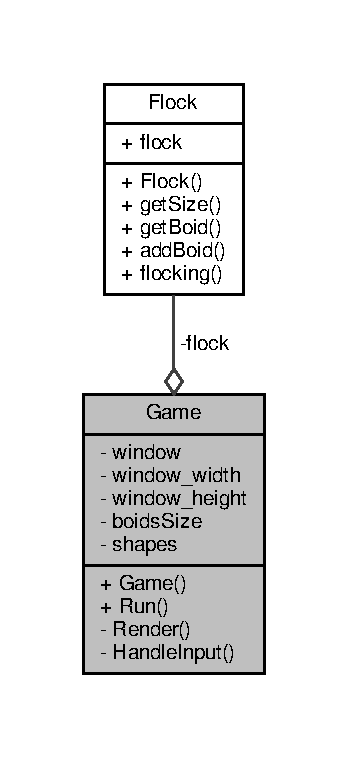
\includegraphics[width=167pt]{class_game__coll__graph}
\end{center}
\end{figure}
\subsection*{Public Member Functions}
\begin{DoxyCompactItemize}
\item 
void {\bfseries Run} ()\hypertarget{class_game_a96341ca5b54d90adc3ecb3bf0bcd2312}{}\label{class_game_a96341ca5b54d90adc3ecb3bf0bcd2312}

\end{DoxyCompactItemize}
\subsection*{Private Member Functions}
\begin{DoxyCompactItemize}
\item 
void {\bfseries Render} ()\hypertarget{class_game_a0897730fc9fed789f6c0f11d21a0c14a}{}\label{class_game_a0897730fc9fed789f6c0f11d21a0c14a}

\item 
void {\bfseries Handle\+Input} ()\hypertarget{class_game_a6cb82eaece4e30724f3fe4e0d4bde5fc}{}\label{class_game_a6cb82eaece4e30724f3fe4e0d4bde5fc}

\end{DoxyCompactItemize}
\subsection*{Private Attributes}
\begin{DoxyCompactItemize}
\item 
sf\+::\+Render\+Window {\bfseries window}\hypertarget{class_game_a223de215aeb661cd423ac145756cc730}{}\label{class_game_a223de215aeb661cd423ac145756cc730}

\item 
int {\bfseries window\+\_\+width}\hypertarget{class_game_ad858cf9f4668f739c4556cd9fcc8a482}{}\label{class_game_ad858cf9f4668f739c4556cd9fcc8a482}

\item 
int {\bfseries window\+\_\+height}\hypertarget{class_game_ad81c3b9b3e2a80b6d27c84e4a9f4eb31}{}\label{class_game_ad81c3b9b3e2a80b6d27c84e4a9f4eb31}

\item 
\hyperlink{class_flock}{Flock} {\bfseries flock}\hypertarget{class_game_ad3e8ecf088a5e6abccd1b4fb5b6533a6}{}\label{class_game_ad3e8ecf088a5e6abccd1b4fb5b6533a6}

\item 
float {\bfseries boids\+Size}\hypertarget{class_game_a3e6bd091af7023583e28ca5d2b8f9ceb}{}\label{class_game_a3e6bd091af7023583e28ca5d2b8f9ceb}

\item 
vector$<$ sf\+::\+Circle\+Shape $>$ {\bfseries shapes}\hypertarget{class_game_abb3836ccb90742ca64267fec2fac57cb}{}\label{class_game_abb3836ccb90742ca64267fec2fac57cb}

\end{DoxyCompactItemize}


\subsection{Detailed Description}
\hyperlink{class_game}{Game} handles the instantiation of a flock of boids, game input, asks the model to compute the next step in the stimulation, and handles all of the program\textquotesingle{}s interaction with S\+F\+ML. 

The documentation for this class was generated from the following file\+:\begin{DoxyCompactItemize}
\item 
Game.\+h\end{DoxyCompactItemize}

\hypertarget{class_pvector}{}\section{Pvector Class Reference}
\label{class_pvector}\index{Pvector@{Pvector}}


{\ttfamily \#include $<$Pvector.\+h$>$}



Collaboration diagram for Pvector\+:
\nopagebreak
\begin{figure}[H]
\begin{center}
\leavevmode
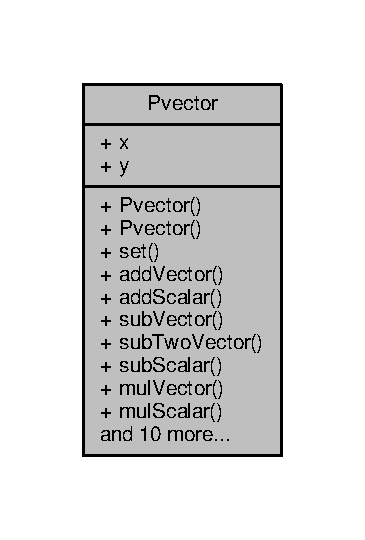
\includegraphics[width=175pt]{class_pvector__coll__graph}
\end{center}
\end{figure}
\subsection*{Public Member Functions}
\begin{DoxyCompactItemize}
\item 
\hyperlink{class_pvector_ada1a9423d48f67838d625ddf62149bcf}{Pvector} (float x\+Comp, float y\+Comp)\hypertarget{class_pvector_ada1a9423d48f67838d625ddf62149bcf}{}\label{class_pvector_ada1a9423d48f67838d625ddf62149bcf}

\begin{DoxyCompactList}\small\item\em Mutator functions. \end{DoxyCompactList}\item 
void \hyperlink{class_pvector_a77eb246570e459227cb4c317af0012b7}{set} (float x, float \hyperlink{class_pvector_ab9d5ab87022aa781382b8eb4b944b375}{y})\hypertarget{class_pvector_a77eb246570e459227cb4c317af0012b7}{}\label{class_pvector_a77eb246570e459227cb4c317af0012b7}

\begin{DoxyCompactList}\small\item\em Scalar functions scale a vector by a float. \end{DoxyCompactList}\item 
void {\bfseries add\+Vector} (\hyperlink{class_pvector}{Pvector} v)\hypertarget{class_pvector_aacdb0c22529bdfa27907013843f78963}{}\label{class_pvector_aacdb0c22529bdfa27907013843f78963}

\item 
void {\bfseries add\+Scalar} (float x)\hypertarget{class_pvector_ab130e1e66e4a33ecf370203e43de191c}{}\label{class_pvector_ab130e1e66e4a33ecf370203e43de191c}

\item 
void {\bfseries sub\+Vector} (\hyperlink{class_pvector}{Pvector} v)\hypertarget{class_pvector_a11ea8cbdc8cc308d5509d5bb85142001}{}\label{class_pvector_a11ea8cbdc8cc308d5509d5bb85142001}

\item 
\hyperlink{class_pvector}{Pvector} {\bfseries sub\+Two\+Vector} (\hyperlink{class_pvector}{Pvector} v, \hyperlink{class_pvector}{Pvector} v2)\hypertarget{class_pvector_a255e0fda569608930ed7986763f6ab85}{}\label{class_pvector_a255e0fda569608930ed7986763f6ab85}

\item 
void {\bfseries sub\+Scalar} (float x)\hypertarget{class_pvector_a0b07f3f6bbdf88179a0aac0bc58b73e1}{}\label{class_pvector_a0b07f3f6bbdf88179a0aac0bc58b73e1}

\item 
void {\bfseries mul\+Vector} (\hyperlink{class_pvector}{Pvector} v)\hypertarget{class_pvector_a70d8afa3b3b30c4c0877bdac66ad5e4a}{}\label{class_pvector_a70d8afa3b3b30c4c0877bdac66ad5e4a}

\item 
void {\bfseries mul\+Scalar} (float x)\hypertarget{class_pvector_aca5515b7c409f641c5565ca0f5bb2940}{}\label{class_pvector_aca5515b7c409f641c5565ca0f5bb2940}

\item 
void {\bfseries div\+Vector} (\hyperlink{class_pvector}{Pvector} v)\hypertarget{class_pvector_aa855eaf087ce971b0aac806aa486793d}{}\label{class_pvector_aa855eaf087ce971b0aac806aa486793d}

\item 
void {\bfseries div\+Scalar} (float x)\hypertarget{class_pvector_a3d60b718b1d2434e52e45a83ea568baf}{}\label{class_pvector_a3d60b718b1d2434e52e45a83ea568baf}

\item 
void \hyperlink{class_pvector_a2c31c0b80bab261fe888395f781328f1}{limit} (double max)\hypertarget{class_pvector_a2c31c0b80bab261fe888395f781328f1}{}\label{class_pvector_a2c31c0b80bab261fe888395f781328f1}

\begin{DoxyCompactList}\small\item\em calculating functions \end{DoxyCompactList}\item 
float {\bfseries distance} (\hyperlink{class_pvector}{Pvector} v)\hypertarget{class_pvector_ad756657de9657b79cf6889ca3161c64e}{}\label{class_pvector_ad756657de9657b79cf6889ca3161c64e}

\item 
float {\bfseries dot\+Product} (\hyperlink{class_pvector}{Pvector} v)\hypertarget{class_pvector_a4eecd15faddd549f3d99002c42b846e9}{}\label{class_pvector_a4eecd15faddd549f3d99002c42b846e9}

\item 
float {\bfseries magnitude} ()\hypertarget{class_pvector_a1aa0154d1d3c92a596610fa366fcfe6c}{}\label{class_pvector_a1aa0154d1d3c92a596610fa366fcfe6c}

\item 
void {\bfseries set\+Magnitude} (float x)\hypertarget{class_pvector_a72261b3f2e1fc1851202f9a96abd8dc1}{}\label{class_pvector_a72261b3f2e1fc1851202f9a96abd8dc1}

\item 
float {\bfseries angle\+Between} (\hyperlink{class_pvector}{Pvector} v)\hypertarget{class_pvector_a7c57bb4e92a54b9d3ebb7f2c4c13743f}{}\label{class_pvector_a7c57bb4e92a54b9d3ebb7f2c4c13743f}

\item 
void {\bfseries normalize} ()\hypertarget{class_pvector_af21ee637474eff3c3387a7b7d138004a}{}\label{class_pvector_af21ee637474eff3c3387a7b7d138004a}

\item 
\hyperlink{class_pvector}{Pvector} {\bfseries copy} (\hyperlink{class_pvector}{Pvector} v)\hypertarget{class_pvector_af5e109a5f1261c4ee69b6f213d7d6154}{}\label{class_pvector_af5e109a5f1261c4ee69b6f213d7d6154}

\end{DoxyCompactItemize}
\subsection*{Public Attributes}
\begin{DoxyCompactItemize}
\item 
float {\bfseries x}\hypertarget{class_pvector_a7ba0ffff299fbf5e127d1849a9c5c87a}{}\label{class_pvector_a7ba0ffff299fbf5e127d1849a9c5c87a}

\item 
float \hyperlink{class_pvector_ab9d5ab87022aa781382b8eb4b944b375}{y}\hypertarget{class_pvector_ab9d5ab87022aa781382b8eb4b944b375}{}\label{class_pvector_ab9d5ab87022aa781382b8eb4b944b375}

\begin{DoxyCompactList}\small\item\em Constructors. \end{DoxyCompactList}\end{DoxyCompactItemize}


\subsection{Detailed Description}
The \hyperlink{class_pvector}{Pvector} class implements Euclidian vectors -- that is, each vector has both a magnitude and a direction. We use Pvectors for implementing movement and the three \hyperlink{class_boid}{Boid} rules -- cohesion, separation, and matching velocity through the use of acceleration, force, and velocity vectors. 

The documentation for this class was generated from the following file\+:\begin{DoxyCompactItemize}
\item 
Pvector.\+h\end{DoxyCompactItemize}

%--- End generated contents ---

% Index
\backmatter
\newpage
\phantomsection
\clearemptydoublepage
\addcontentsline{toc}{chapter}{Index}
\printindex

\end{document}
